\documentclass[11pt]{article}
\usepackage{float}
\usepackage{graphicx}
\usepackage{xcolor}
\usepackage{listings}
\usepackage{enumerate}
\usepackage[backend=bibtex]{biblatex}

\usepackage{comment}

\usepackage{amssymb}
\usepackage{physics}

\usepackage{xepersian}
\settextfont[Scale=1.2]{IRLotus}
\title{برتریِ کوانتومی، کوانتومِ برتری}
\author{سید سجاد کاهانی \\ sskahani@ce.sharif.edu}
\date{۲۷ مهر ۱۳۹۸}
\addbibresource{references.bib}

\begin{document}
\maketitle
ویراستاران: علی بهجتی، امیررضا نگاری، مهرگان درودیانی

خبری که احتمالاً شنیده‌اید، این است که گوگل به برتریِ کوانتومی رسید، چیزی که به‌نظر می‌رسد اتفاقِ شگرفی باشد. حداقل از حجمِ خبرهایی که در این‌باره نوشته شده این‌طور به نظر می‌رسد.

به طورِ خلاصه خبر این بود که گوگل، با کامپیوتری که قبلاً ساخته‌بود، توانسته کاری تقریباً غیرممکن را انجام دهد و از درستیِ نتیجهٔ آن مطمئن شود. کارِ تقریباً غیرممکن یعنی کاری که هیچ کامپیوترِ معمولی‌ای نمی‌تواند به این زودی‌ها انجامش دهد.

جزئیاتِ خبر، حتی اگر از نظرِ ریاضی برای ما قابلِ فهم باشد، برای یک مهندسِ کامپیوتر چندان هیجان‌انگیز به نظر نمی‌آیند. اما همچنان برای همهٔ‌ ما جذاب است که سر از کارِ این کامپیوترهای کوانتومی دربیاوریم. برای همین در چند قصهٔ بی‌ربط به هم، از بنیان‌های مکانیکِ کوانتومی، به مسئله می‌رسیم.

\section{گربهٔ آقای شرودینگر}

\begin{figure}[H]
\centering
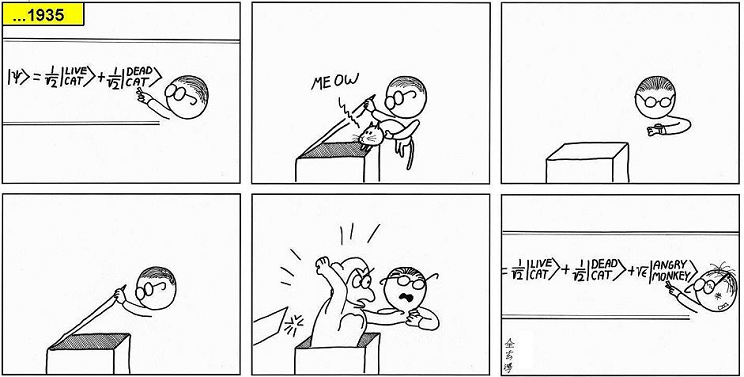
\includegraphics[width=0.9\textwidth]{res/schrodinger_miscalc.png}
\caption{از \cite{goose}}
\end{figure}

فیزیکِ کوانتوم، تاریخچهٔ پیچیده و طولانی‌ای دارد که گفتنش حداقل به ملموس‌تر شدنِ مطلب، کمکِ زیادی می‌کند. اما به خاطرِ بی‌سوادیِ نویسنده در تاریخِ کوانتوم، خودِ کوانتوم و البته برای ایجاز، از گفتنِ آن می‌پرهیزیم.

داستان را با گربهٔ مظلومِ آقای شرودینگر شروع می‌کنیم
\footnote{دربارهٔ مظلومیتِ گربهٔ آقای شرودینگر همین بس که هدفش بیانِ تناقض در تفسیرِ کپنهاگیِ مکانیکِ کوانتومی بوده \cite{schrodinger} که اکنون ما دقیقاً برای آموزشِ تفسیرِ کپنهاگی از آن بهره می‌جوییم.}
 که در جعبه‌ای‌ست که هیچ ارتباطی با بیرون ندارد. در آن جبعهٔ، یک ظرفِ سم وجود دارد که با یک تابشِ رادیواکتیو (یا هر پدیدهٔ کوانتومی‌ای که شما دوست دارید) فعال می‌شود. از مکانیکِ کوانتومی برمی‌آید که این گربه حالا هم مرده و هم زنده‌است. (یا به عبارتِ بهتر برهم‌نهیِ دوحالتِ مرده و زنده)

\begin{center}
\begin{minipage}[H]{0.6\textwidth}
\emph{
برای این قسمت خوب است با فضای برداری آشنا باشید. فضای برداری را می‌توانید از یک جزوهٔ جبرخطی یا یک ویدیوی یوتوب یاد بگیرید. یا حتی اگر می‌خواهید خیلی‌خیلی بیشتر بدانید فضای هیلبرت را یاد بگیرید.
}
\end{minipage}
\end{center}
\vspace{3mm}

برای نمایشِ ریاضی‌ این وضعیت، یک فضای برداریِ دوبعدیِ مختلط بگیریم که پایه‌های آن 
$\va{e_1}$ (به معنای سلامت گربه) و 
$\va{e_2}$  (به معنای پرپر شدنِ گربه)
 هستند که برهم عمودند، 
\footnote{
اگر بخواهیم مته به خشخاش \footnotemark بگذاریم، در اصل باید حالت‌های کلِ سیستمِ داخلِ جعبه، یعنی سم و گربه را به شکلِ توؤمان بیان کنیم. یعنی 
$\va{e_1}$ می‌شود 
«گربه سالم است و سم منتشر نشده» و 
$\va{e_2}$ هم حالتِ «گربه پرپر شده و سم منتشر شده» }
\footnotetext{
محمدامین خشخاشی‌مقدم، ورودی ۹۳ مهندسیِ کامپیوتر
}
حالا گربه در حالتِ زیر قرار دارد.

\[ \text{\lr{state}} = \frac{1}{\sqrt{2}} (\va{e_1} + \va{e_2}) \]

که به احترامِ آقای دیراک برای نشان دادنِ بردارهایمان به جای $\va{v}$ از $\ket{v}$ استفاده می‌کنیم.

در حالتِ کلی، این‌طور می‌گوییم که اگر سیستمی قبلاً، یکی از حالت‌های 
$Q = \{ q_1\dots q_n \}$
را به خود اختصاص می‌داد، در مکانیکِ کوانتومی، حالتِ سیستم، برداری‌ست با اندازهٔ یک در فضای مختلطی که اعضای پایهٔ متعامدش
$\ket{q_1}\dots\ket{q_n}$
هستند، یعنی عضوی از مجموعهٔ 
$\mathbb{C}^Q$.

همین‌طور، گذارِ خودبه‌خودیِ یک سیستم، که قبلاً می‌شد با تابعی از $Q$  به $Q$ بیان شود، در مکانیکِ کوانتومی با یک تبدیلِ خطی در فضای برداریِ حالت‌ها بیان می‌شود. این تبدیل اندازهٔ بردار را حفظ می‌کند (چون گفتیم هر بردارِ حالتی اندازه‌ای برابرِ یک دارد) پس یکانی‌ست.

اکنون اگر درِ جعبه را باز کنیم با یکی از این دو واقعیت روبه‌رو می‌شویم که گربه زنده است یا گربه پرپر شده. یعنی هر بردارِ دلخواهی که وضعیتِ گربه پیش از باز شدن بوده، باید به یکی از پایه‌ها تبدیل شود‌
\footnote{رمبیدن که ترجمهٔ collapse است فعلِ صحیح‌تری از تبدیل شدن است،‌ اما برای حفظِ خوانایی از آن استفاده نمی‌کنیم.}. 
با بی‌خیال شدنِ جزئیات و کلیات، احتمالِ این‌که بعد از باز کردنِ درِ جعبه‌، گربه‌ از حالتِ $\ket{v}$ به عضوِ پایهٔ $\ket{q_i}$ تبدیل شود و  حالتِ $q_i$ را مشاهده کنیم، می‌شود
\[ \Pr(q_i) = |\braket{v}{q_i}|^2 \]

که این علامتِ 
$\braket{a}{b}$
 همان ضربِ داخلی‌ست.

\section{از دکتر آبام تا دکتر وزیرانی}

\begin{center}
\begin{minipage}[H]{0.6\textwidth}
\emph{
برای این قسمت خوب است با ماشینِ تورینگ و نمایشِ ریاضیِ آن آشنا باشید. برای این‌کار هم ویدیویی از یوتوب نگاه کنید و هم از روی جزوه یا ویکی‌پدیا، فرمِ ریاضیِ آن را ببینید. همچنین خوب است کلاسِ مسئله‌های $\mathcal{P}$ و $\mathcal{NP}$ را هم از روی یک ویدیوی یوتوب یاد بگیرید.
}
\end{minipage}
\end{center}
\vspace{3mm}

از ماشینِ تورینگ، همین را به خاطرِ بیاورید که تابعی داشت که از $Q \times \Gamma$ که حالت‌ها و الفبای ورودیِ روی نوار هستند، به 
$Q \times \Gamma \times \{L, R\}$
می‌رفت. این تابعِ گذار، مشخص می‌کرد که وقتی در حالتی هست و علامتی را روی نوار می‌بیند، به چه حالتی برود، چه علامتی در جایگاهِ فعلیِ نوار بنویسد و به کدام سمت روی نوار حرکت کند. حالا برای کوتاه‌نویسی این‌دوتا را تعریف می‌کنیم.

\[A := Q \times \Gamma\]
\[B := Q \times \Gamma \times \{L, R\}\]

یکی دیگر از این ماشین‌های خیالی، ماشینِ تورینگِ احتمالاتی‌ست. تابعِ گذارِ این ماشین، احتمالاتی‌ست. یعنی برای هر مرحله، تاس می‌اندازد.

به شکلِ ریاضی‌تر، اگر برای تابعِ گذارِ ماشینِ تورینگ داشتیم 
$\delta: A \rightarrow B$
حالا داریم که
\[ \delta: (A \times B) \rightarrow [0,1] \]
و این تابع، به ازای هر $A$ یک توزیعِ احتمال است که یعنی برای هر عضوِ $A$ مانندِ $a$ داریم
\[ \begin{cases}
  \forall b \in B: \delta(a, b) = \Pr(b) \ge 0 \\
  \sum_{b \in B} \delta(a, b) = \sum_{b \in B} \Pr(b) = 1
\end{cases} \]

اگر چیزی را این ماشینِ تورینگِ احتمالاتی بتواند با احتمالِ بیش‌تر از $\frac{2}{3}$ تشخیص دهد، می‌گوییم آن‌چیز عضوِ کلاسِ
$\mathcal{BPP}$ است و همین اول می‌شود حدس زد که $\mathcal{P} \subseteq \mathcal{BPP}$.
\footnote{یکی از مسئله‌های جالب، با ته‌مایه‌هایی از فلسفه این است که آیا این دو کلاس مساوی هستند یا نه و اگر باشند و نباشند هریک چه معنایی دارد. توضیحاتِ بیشتر را در این مقاله \cite{goldreich} ببینید.}

حالا ماشینِ تورینگِ کوانتومی، احتمالاً یک تابعِ گذار به شکلِ یک تبدیلِ خطی خواهد داشت که اندازه را حفظ می‌کند. آن را به این صورت تعریف می‌کنیم.
\cite{deutsch}
\[ \delta: A \rightarrow \mathbb{C}^{B} \]

این تابع به هرحالتِ $A$ یک بردارِ مخلتط در فضایی با پایه‌های $B$ نسبت می‌دهد. اما می‌دانیم که می‌توانیم در برهم‌نهی‌ای از حالت‌های $A$ باشیم، یعنی حالتمان برداری به نامِ $\ket{\psi}$ عضوِ 
$\mathbb{C}^A$ باشد.
که به شکلِ زیر قابلِ نوشتن است
\[ \ket{\psi} = \sum_{a_i \in A} \beta_i \ket{a_i} \]

حالا در تبدیلِ حالتی که اتفاق می‌افتد، به شکلِ خطی، هریک از مؤلفهٔ‌های $\ket{a_i}$ به بردارِ مربوط، یعنی $\delta(a_i)$ می‌رود. پس گذار به این شکل انجام می‌شود.

\[ \ket{\psi} \rightarrow \sum_{a_i \in A} \beta_i \delta(a_i) \]


دربارهٔ حفظ شدنِ اندازهٔ بردارِ حالت نیز باید بگوییم اگر حالت‌های یک ماشین (شاملِ محلِ نشان و وضعیتِ نوار و وضعیتِ ماشین و چیزهای دیگر) را مجموعهٔ $S$ بنامیم، در هر مرحله، تحولی که صورت می‌گیرد، باید اندازهٔ بردارهای فضای 
$\mathbb{C}^S$ 
را حفظ کند.

می‌دانیم که در کوانتوم، در انتها، با اندازه‌گیری (باز کردنِ جعبه)، بردارِ حالت به یکی از پایه‌ها تبدیل می‌شود، که این یک فرایندِ احتمالاتی‌ست. پس برای همین، مشابهِ کلاسِ $\mathcal{BPP}$، تعریف می‌کنیم کلاسِ $\mathcal{BQP}$، شاملِ چیزهایی‌ست که یک ماشینِ کوانتومی با احتمالِ بیشتر از $\frac{2}{3}$ تشخیص می‌دهد. آقایان برنشتاین و وزیرانی اثبات کرده‌اند که 
$\mathcal{BPP} \subset \mathcal{BQP}$.
\cite{bernstein}
 و همچنین اثبات شده که
$\mathcal{NP} \nsubseteq \mathcal{BQP}$
\cite{bennett}

\section{برتریِ کوانتومی، یک برخوردِ‌ صادقانه و مهندسی}

مقالاتِ مختلفِ تئوری \cite{aaronson} و عملی\cite{boxio}، به خاطرِ تفاوتِ دیدگاه‌ها، معمولاً تعاریف و شروطِ مختلفی را برای برتریِ کوانتومی می‌گویند، اما به طورِ کلی، می‌توان این دوشرط را بیان کرد که البته هرکدام قابلِ بحث هستند

محاسباتی طراحی و انجام شود که:
\begin{enumerate}[-]
\item با یک کامپیوترِ کوانتومی قابلِ انجام باشد ولی با کامپیوترِ معمولی غیرِ قابلِ انجام باشد. (مثلاً زمانِ زیادی طول بکشد یا حافظهٔ زیادی لازم داشته‌باشد)
\item جوابِ مسئله قابلِ ارزیابی باشد.
\end{enumerate}

اگر مسئله‌ای عضوِ $\mathcal{BQP}$ باشد و در عینِ حال عضوِ $\mathcal{NP}$ باشد (و طبیعتاً عضوِ $\mathcal{P}$ نباشد)، به این معنی‌ست که مطمئنیم وقتی اندازهٔ مسئله از حدی بزرگ‌تر شود
 کامپیوترهای کوانتومی آن را سریع‌تر حل می‌کنند و همچنین در زمانِ تقریباً کوتاهی می‌توانیم پاسخِ این مسئله را با یک کامپیوترِ معمولی ارزیابی کنیم.

پس احتمال می‌دهیم مسئله‌هایی از این دست نظیرِ «تجزیهٔ عدد به عواملِ اول» یکی از کاندیداهای خوب برای نمایشِ برتریِ کوانتومی باشند. اما در حقیقت، بیشترِ طرح‌هایی که برای نمایشِ برتریِ کوانتومی ارائه می‌شوند، روی مسئله‌های متفاوتی نظیرِ نمونه‌برداری از یک توزیع تمرکز دارند. چرا؟\cite{aaronson}

\begin{enumerate}[-]
\item کامپیوترِ کوانتومیِ همه‌کارهٔ بدونِ نویزِ درست‌حسابی نداریم.
\item فکر می‌کنیم که مسئلهٔ تولیدِ اعدادِ تصادفی خیلی‌خیلی سخت‌تر از یک تجزیهٔ عدد برای کامپیوترهای معمولی‌ست.
\item
البته که علایقِ فیزیک‌دانان در طرحِ این مسائل دخیل بوده‌است. 
\end{enumerate}

\section{مسئلهٔ مدارِ تصادفی}
یک مدارِ منطقیِ معمولی، یک تابعی‌ست که از $\{0, 1\}^N$ به $\{0, 1\}^M$ می‌رود. حالا یک مدارِ منطقیِ کوانتومی (که لزوماً برگشت‌پذیر هم هست) یک تبدیلِ خطیِ یکانی‌ست، در فضایی که  پایه‌هایش $\{0, 1\}^N$، یعنی رشته‌های $N$-بیتی اند. به این فضا،‌ فضای $N$-کیوبیتی و به این مدار نیز مدارِ $N$-کیوبیتی یا گیت $N$-کیوبیتی می‌گوییم.

فرض کنید که حالتِ $\ket{\psi_0}$ را به‌عنوانِ ورودی به مدارِ کوانتومیِ $U$ داده‌ایم، سپس اندازه‌گیری‌ای کرده‌ایم که نتیجه‌ش یکی از اعدادِ $1\dots 2^N$ مانندِ $q$ است. احتمالِ هر خروجی را 
$\Pr_\text{ideal}(q|U)$
می‌نامیم.

همچنین در نظر بگیرید، برای ساختِ مدارِ $U$، مدارهای یک‌ورودی-یک‌خروجی و دوورودی-دوخروجی را به شکلِ تصادفی ترکیب کرده‌ایم. یعنی با ترکیب کردنِ تعدادی از مدارهای ساده و کوچک -که مشخص هستند-، با یک الگوی تصادفی، یک مدارِ تصادفیِ بزرگ ساخته‌ایم.

اگر به این مدارِ تصادفیِ $U$، ورودی‌ای بدهیم و خروجیِ آن را اندازه بگیریم، $q$ عددی از توزیعی خاص خواهدبود. نمونه‌برداری از این توزیع، مسئلهٔ ماست.

\[ \Pr(q) = \sum_U \Pr_\text{ideal} (q|U) \Pr(U) \]

شبیه‌سازیِ این فرایند و نمونه‌برداری از توزیعِ آن، توسطِ کامپیوترهای معمولی کارِ بسیار مشکلی خواهدبود. \cite{boxio} این به نظر می‌رسد که فوق‌العاده‌ است، اما باید به سؤالات پاسخ داد:
\begin{enumerate}[-]
\item از کجا مطمئنیم این کار برای یک کامپیوترِ معمولی به اندازهٔ کافی مشکل است. شاید فقط ما بلد نیستم.
\item از کجا مطمئن شویم واقعاً کامپیوترِ کوانتومی‌مان درست کار می‌کند و نمونه‌ها واقعاً از توزیعِ مذکور هستند؟ 
\end{enumerate}

در پاسخ به سؤالِ اول، باید صادقانه بگوییم که نمی‌دانیم.
\cite{aaronson}
این بیشتر شبیهِ یک تحدی‌ست که ادعا می‌کنیم این محاسبات را هیچ‌کسی نمی‌تواند انجام دهد و باید منتظر بمانیم و شاید مردی از خویش برون آید و الگوریتمی نو دراندازد و کاری بکند.

پاسخ دادن به سؤالِ دوم اما چندان آسان نیست (بوی پیچاندن می‌آید)، پاسخ کوتاه این است که نمی‌توانیم مطمئن شویم \cite{aaronsonfaq} و پاسخِ بلند خودش قصهٔ طولانی‌ای‌ست که در ادامه می‌گوییم.
\section{و ارزیابی‌ش}
\begin{center}
\begin{minipage}[H]{0.6\textwidth}
\emph{
برای این قسمت، لازم است که آمار و احتمال بلد باشید. تقریباً به اندازهٔ درسِ آمار و احتمال که به شکلِ مرسوم ارائه می‌شود.
}
\end{minipage}
\end{center}
اگر مدارِ تصادفیِ $U$ که در قسمتِ قبل گفتیم، با احتمالِ $F$، با خطا عمل کند، آنگاه می‌توان این فرایند را به این صورت بیان کرد

\[ \Pr_\text{experiment}(q|U) = F \Pr_\text{ideal}(q|U) + (1 - F) \Pr_\text{error}(q|U) \]

که در $\Pr_\text{error}$ توزیعِ نتیجهٔ آزمایش درصورتِ بروزِ خطاست.

با دو فرضِ  زیر می‌توان سنجه‌ای میزانِ خطا پیدا کرد.
\begin{enumerate}[-]
\item
با توجه به این‌که این احتمالات ناشی از رخدادهای کوانتومی هستند خطاهایی که مدارهای مختلف رخ می‌دهند، در مجموعِ همهٔ مدارها، اریب نباشند و تقارنی نسبت به $q$ها داشته‌باشند. یعنی به طورِ میانگین (برای همهٔ $U$ها) این توزیع، یکنواخت باشد. \cite{google}

\[ \mathbb{E}_U[\Pr_\text{error}(q|U)] = \frac{1}{2^N} \]

\item
با توجه به شیوه‌ای که این مدارهای تصادفی را می‌سازیم، نتایجِ اندازه‌گیری از توزیعِ پورتر-توماس
\footnote{
این توزیع که در ابتدا از داده‌های یک آزمایش مربوط به نوسان‌های واکنش‌های هسته‌ای به دست آمده‌است \cite{porter} و بعدها در مسئله‌های مختلفِ آشوبِ کوانتومی موردِ توجه قرار گرفته، با توجه به آشوبناکِ بودنِ این مسئله و نتایجِ شبیه‌سازی‌ها \cite{boxio} برای حالتِ ایده‌آلِ این آزمایش (با تعدادِ مراحلِ کافی) معتبر می‌باشد.
} تبعیت کند.

این توزیع بیان می‌کند که برای یک $q$ دلخواه، $U$ یک متغیرِ تصادفی‌ست پس $p = \Pr_\text{ideal}(q|U)$ نیز یک متغیرِ تصادفی‌ست که تابعِ چگالیِ احتمالِ آن به شکلِ زیر است
\footnote{
این‌که $f(p)$ برای $p > 1$ مقداری بزرگ‌تر از صفر دارد و این شاید نادرست به نظر برسد، اما در شرایطی که $2^N \gg 1$ \cite{google}، این مقدار بسیار ناچیز و تقریباً برابر با صفر است. البته که این صحبت دقیق نیست و تنها برای تقریبِ ذهن است.
}
\[ f(p) = 2^N e^{-2^N p}  \]
\end{enumerate}

با این دوفرض، می‌توانیم به این معادله برسیم
\[ \mathbb{E}_U\Big[\mathbb{E}_\text{experiment}[2^N \Pr_\text{ideal}(q | U) - 1]\Big] = F \]


و این یعنی با دانستنِ مقدارِ 
$\Pr_\text{ideal}(q|U)$
و با نمونه‌برداری از آن، به ازای $U$ها و $q$های مختلف (برای $S_U$تا مقدار از $U$ و هرکدام با $S_q$ مقدار از $q$)، طبقِ قانونِ اعدادِ بزرگ، تخمینی از $F$ را به دست می‌آوریم.

\[ \frac{1}{S_U S_q} \sum_U \sum_q (2^N \Pr_{\text{ideal}}(q |U) - 1) = F + \mathcal{O}(\frac{1}{\sqrt{S_U S_q}}) \]

و همان‌طور که پیش‌تر پارامتر $F$ را تعریف کرده‌ایم، احتمالِ سلامتِ آزمایش است، که معیاری از کیفیتِ انجامِ آزمایش است.

اما حساب کردنِ $\Pr_\text{ideal}(q|U)$ مستلزمِ شبیه‌سازیِ کاملِ مدار در کامپیوترِ معمولی‌ست. این یعنی تا جایی که امکانِ شبیه‌سازیِ مسئله در کامپیوتر وجود دارد، می‌توانیم آن را ارزیابی کنیم.

ولی داستان به همین‌جا ختم نمی‌شود. گوگل، ابتدا از طریقِ بررسیِ خطاها، پیش‌بینیِ اولیه‌ای از کیفیتِ نمونه‌برداری در شرایط مختلف (تعدادِ کیوبیت‌ها و تعداد مراحل شرایط مسئله هستند) به دست می‌آورد. سپس، چند نوع مدارِ تصادفیِ ساده‌شده نیز طراحی می‌کند و در نهایت نشان می‌دهد که کیفیتِ مدارهای ساده‌شده با مدارِ اصلی با پیش‌بینی‌ برابر است. سپس، با افزایشِ تعدادِ مراحل (سخت‌تر کردنِ مسئله) مدارهای ساده‌شده همچنان منطبق بر شبیه‌سازی‌‌ها هستند اما ارزیابیِ کیفیتِ مدارِ اصلی دیگر غیرممکن است و این یعنی به برتریِ کوانتومی دست پیدا کرده‌ایم. \cite{google}

\begin{figure}[H]
\centering
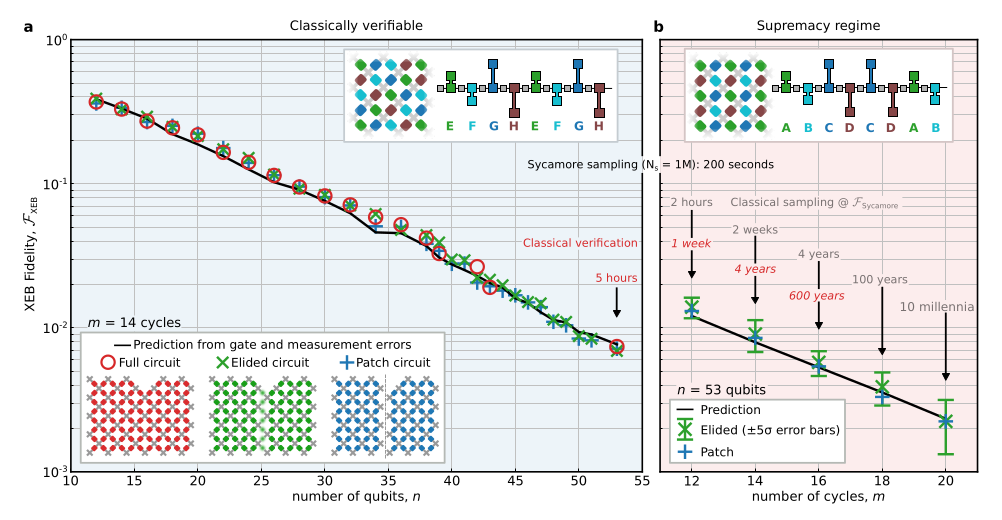
\includegraphics[width=0.9\textwidth]{res/google_supremacy.png}
\caption{شکلِ برتریِ کوانتومی در گزارشِ گوگل \cite{google}}
\end{figure}

\section{کازینوی مونته‌کارلو}

\begin{center}
\begin{minipage}[H]{0.6\textwidth}
\emph{
برای این قسمت لازم است با مفهومِ تانسور، ضربِ تانسوری، ضربِ ماتریسی و روش‌های نمونه‌برداری آشنا باشید. دانستنِ مفهومِ ضربِ تانسوری تقریباً حیاتی‌ست، پس یوتوب را باز کنید.}
\end{minipage}
\end{center}

\begin{figure}[H]
\centering
\includegraphics[width=0.6\textwidth]{res/casino_2.jpg}
\caption{کازینوی بزرگِ مونته‌کارلو، شاهزاده‌نشینِ موناکو}
\end{figure}

یکی از قسمت‌های جذاب و قابلِ فهمِ مسئله این است که چه کدی توی کامپیوترهای معمولی‌مان بزنیم که همین مسئله را (در ابعادِ کوچک) شبیه‌سازی کند؟

برای یک شبیه‌سازیِ کاملاً واقعی، پنج کیوبیت را در نظر بگیرید، که حالتِ آن‌ها تشکیلِ یک بردارِ مختلط در فضای $2^5$-بعدی (یا یک تانسورِ 
$2\times 2\times 2\times 2\times 2$
) می‌دهد. فرض کنید حالتِ اولیهٔ این پنج کیوبیت 
$\ket{00000}$
باشد، یعنی مقدارِ آن بردار برابرِ
$ (1, 0, \dots 0) $
خواهد بود.

در ساختارِ تانسوری، اگر بخواهیم یک گیتِ تک‌کیوبیتی را (که یه ماتریس 
$2 \times 2$
است) روی کیوبیتِ سوم اعمال کنیم، باید یک ضربِ ماتریسی برروی بعدِ سومِ تانسورِ حالتمان انجام دهیم. این کدِ واقعیِ پایتون همین‌ کار را می‌کند.


\lstset{language=Python, 
	backgroundcolor=\color{gray!10!white},
	breaklines=true,
	frame=single,
	commentstyle=\color{gray!60!black},
	stringstyle=\color{purple},
	numberstyle=\tiny\color{gray},
	keywordstyle=\color{green!50!black},
  identifierstyle=\color{blue},
	numbers=left,
	numbersep=5pt,
	showstringspaces=false,
	rulecolor=\color{gray},
	tabsize=4,
  basicstyle=\ttfamily\small
}
        
\begin{latin}
\begin{lstlisting}
import numpy

state_shape = (2, 2, 2, 2, 2)
state = np.reshape(np.array([1] + 31 * [0]), state_shape)

# a valid quantum state must have norm = 1
assert(np.linalg.norm(state) == 1.0)

gate = np.matrix([[0, 1j], [-1j, 0]])

# a valid quantum gate must be unitary (maintains norm)
assert(np.all(np.matmul(gate.H, gate) == np.identity(2)))

# apply gate on 3th qubit (2nd if we start from 0) 
np.tensordot(gate, state, axes=(1, 2))

\end{lstlisting}
\end{latin}

حالا به سراغِ دستورالعملِ گوگل برای مدارِ تصادفی می‌رویم.

\begin{figure}[H]
\centering
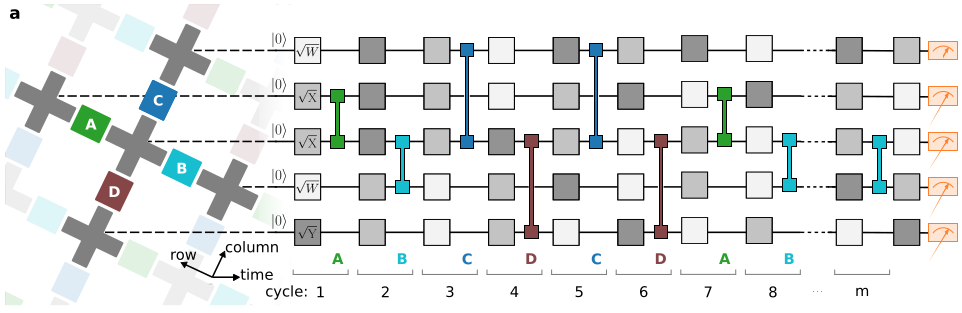
\includegraphics[width=0.9\textwidth]{res/google_circuit.png}
\label{fig:google_circuit}
\caption{الگوی گوگل در ایجادِ مدارِ تصادفی \cite{google}}
\end{figure}

این دستورالعمل، از $m$مرحله تشکیل شده که در هرمرحله این دو فرایند انجام می‌شود

\begin{enumerate}[-]
\item 
به ازای هرکدام از کیوبیت‌ها، به شکلِ تصادفی یکی از سه گیتِ $\sqrt{X}, \sqrt{Y}, \sqrt{W}$
\footnote{مهم نیست این رادیکال‌ها و نامگذاری‌ها چه معنی‌ای می‌دهند و چه دلیلی دارند، ما می‌دانیم هر گیتِ تک‌کیوبیتی، یک ماتریسِ 
$2\times 2$
 است و تنها مقدارِ این ماتریس‌ها را بدانیم.}
 را انتخاب می‌کنیم و اعمال می‌کنیم. اگر در مرحلهٔ پیش یکی از این سه‌گیت را روی این گیت اثر داده‌ایم، از انتخاب‌هایمان حذفش می‌کنیم و از بینِ دو گیتِ باقی‌مانده یکی را برمی‌گزینیم.

\item
مطابقِ الگوی هرمرحله، برروی زوج کیوبیت‌های مشخص‌شده توسط الگو، گیتِ دوکیوبیتی‌ای را که $\text{fSim}(\pi/2, \pi/6)$ نام دارد، اعمال می‌کنیم.
\footnote{یک گیت دوکیوبیتی یک تبدیلِ خطی برروی فضای 
$2 \times 2$
بعدی‌ست. به عبارتِ دیگر، یک ماتریسِ 
$4 \times 4$
 است.}
\end{enumerate}

الگوی هر مرحله، یکی از حروف A تا H می‌تواند باشد که مشخص می‌کند که برروی کدام زوج کیوبیت‌ها این گیتِ دوکیوبیتی اثر کند. (مانند شکل \ref{fig:google_circuit}) دنبالهٔ الگوی مرحله‌ها در این موردِ شبیه‌سازیِ ما عبارتِ تکرارشوندهٔ 
\lr{ABCDCDAB}
است.\cite{google}
 
 مقدارِ این گیت‌ها به ترتیب است:
 
\[ \sqrt{X} = \frac{1}{\sqrt{2}} \begin{bmatrix} 1 & - i \\ -i & 1 \end{bmatrix} \]
 
\[ \sqrt{Y} = \frac{1}{\sqrt{2}} \begin{bmatrix} 1 & - 1 \\ 1 & 1 \end{bmatrix} \]

\[ \sqrt{W} = \frac{1}{\sqrt{2}} \begin{bmatrix} 1 & - \sqrt{i} \\ \sqrt{-i} & 1 \end{bmatrix} \]

\[ \text{fSim}(\pi/2, \pi/6) = \begin{bmatrix} 
1 & 0 & 0 & 0 \\
0 & 0 & -i & 0 \\
0 & -i & 0 & 0 \\
0 & 0 & 0 & e^{-i\frac{\pi}{6}} \end{bmatrix} \]

در مرحلهٔ آخر، تنها گیتِ یک‌کیوبیتی اعمال می‌کنیم و سپس به سراغِ اندازه‌گیری می‌رویم.

برای اندازه‌گیریِ این بردارِ حالت که به شکلِ 
$2\times 2\times 2\times 2\times 2$
است، برای هرمؤلفهٔ آن که $v$ باشد داریم 
$|v|^2$
احتمالِ رخدادِ رشته‌بیتِ هم‌ارزِ آن مؤلفه است. حالا کافی‌ست از این توزیع نمونه‌هایی را برداریم و پارامترِ $F$ را که در قسمتِ قبل معرفی کردیم برای آن‌ها محاسبه کنیم.

و در نهایت، با کدِ زیر می‌خواهیم صد بار،  با شش مرحله مدارهای تصادفی‌ای بسازیم و هربار با ده‌بار نمونه‌برداری از خروجی، پارامترِ $F$ را تخمین بزنیم.

\begin{latin}
\begin{lstlisting}
import numpy as np
from random import choice

n = 5
cycles = 6
state_shape = (2, 2, 2, 2, 2)

# define single-qubit gates
xsqrt = np.array([[1, -1j], [-1j, 1]]) / np.sqrt(2)
ysqrt = np.array([[1, -1], [1, 1]]) / np.sqrt(2)
wsqrt = np.array([[1, -np.sqrt(1j)], [np.sqrt(-1j), 1]]) / np.sqrt(2)

single_gates = [xsqrt, ysqrt, wsqrt]

# define double-qubit gates
double_gate = np.array([[1, 0, 0, 0], \
                        [0, 0, -1j, 0], \
                        [0, -1j, 0, 0], \
                        [0, 0, 0, np.exp(1j * np.pi/6)]])
double_gate = np.reshape(double_gate, (2, 2, 2, 2))

# double-qubit gate pattern (from shape) ABCDCDAB
pattern = [(1,2), (2,3), (0,2), (2,4), (0,2), (2,4), (1,2), (2,3)]

# sample from different 100 random circuits
samples_U = 100

# list of F values
fs = []

for _ in range(samples_U):
  last_applied_gate = [None] * n

  # define input state
  state = np.reshape(np.array([1] + 31 * [0]), state_shape)

  # iterate over cycles
  for c in range(cycles):
    # iterate over qubits to apply single gates 
    for i in range(n):
      # apply a random gate on ith qubit
      gate = choice([g for g in single_gates if np.all(g != last_applied_gate[i])])
      state = np.tensordot(gate, state, axes=(1, i))
      
    # apply double-qubit gate
    state = np.tensordot(double_gate, state, axes=((2,3), pattern[c % len(pattern)]))
    
  # last half cycle
  for i in range(n):
    gate = choice([g for g in single_gates if np.all(g != last_applied_gate[i])])
    state = np.tensordot(gate, state, axes=(1, i))
    
  # let's dice!
  ps = (abs(state)**2).flatten()
  # number of samples from output of this circuit
  samples_q = 10
  for _ in range(samples_q):
    fs.append(2**n * np.random.choice(ps, p=ps) - 1)
  
print('F = ', np.mean(fs), '±', np.std(fs) / np.sqrt(len(fs) - 1))
\end{lstlisting}
\end{latin}

نتیجهٔ اجرای این کد، برای من این شد، انتظار داشتیم چند بشود؟

\[ F =  0.98 \pm 0.05 \]

بعد از این اتفاق‌ها آی‌بی‌ام ادعا کرده که برتریِ کوانتومی رخ نداده و این محاسبات را می‌توان در طیِ دو روز با یک سوپرکامپیوتر انجام داد. \cite{ibm}

(امروز که این نوشته تمام شد سالگردِ مرتضی کیوان بود. کاشکی به جای این‌همه حرفِ مفت، فقط می‌نشستیم و یادی از او می‌کردیم)

\section*{مراجع}
\begin{latin}
\printbibliography[heading=none]
\end{latin}

\end{document}
